\chapter{Experiments}
\label{chap:experiments}

All last chapters refer to the theory and name some theoretical implementation-details, all to verify the developed procedure.
However, this chapter presents some results to validate, that the distribution of found paths really improves.

\section{The testing-machine and simulation-setup}

    Firstly, the used machine runs an AMD Ryzen 7 3700X 8-Core Processor and has \si{\num{32} \giga\byte} of RAM built in.
    The operation-system is Arch Linux [x86\_64] with the kernel 5.7.9-arch1-1 installed.
    The used code for this thesis can be found in \cite{github:dominicparga/osmgraphing} and is implemented in Rust.
    Python is used for the visualization.
    Internally, this repository uses \cite{github:lesstat/multi-ch-constructor} (written in C++) for the \gls{contraction-hierarchies} as git-submodule and \cite{github:lesstat/nd-triangulation} for memory-management of the convex-hull.
    The latter is basically a Rust-wrapper for CGAL (C++).
    Please note, that the implementation is not tested for deterministic execution, but results are sufficiently similar.
    Reasons for non-determinism could be multithreaded parsing and multithreaded graph-contraction, because edges don't come with an unique identifier and thus gets one after first parsing.

    \todo{%
        TODO @Florian

        Passt der vorherige Satz mit der graph-contraction bzgl Determinismus so?
        Die "graph-contraction" bezieht sich auf den multi-ch-constructor, das parsing auf meinen pbf-parser, der multithreaded einliest, was aber nicht mein Code ist.
        Vielleicht werden hier edges durcheinander geschmissen, die anfangs natürlich keine ID von pbf-Files mitbringen.
        Ich würde das mit dem Determinismus aber gerne sagen, denn exakte Reproduzierbarkeit der Ergebnisse ist ja dann nicht gegeben.
    }

    Graphs for street-networks are downloaded from \cite{osm}.
    Experiments run on the graph for Isle~of~Man (from March~2020) and on the graph for the German state Saarland (from July~2020).
    Considered \glspl{metric} are travel-distance (all paths tolerated) and travel-time (\si{40 \percent} tolerance on Isle~of~Man, \si{25 \percent} on Saarland).
    A tolerance of \si{25 \percent} refers to a worst-case-scenario of \si{15 \minute} more for originally \si{60 \minute}, which seems to be a good tradeoff.
    However, a tolerance of \si{40 \percent} refers to a worst-case of additional \si{24 \minute} for originally \si{60 \minute}.
    According to a simple Google-maps-query, one of the paths from one end of the island to the other takes $\approx \si{45 \minute}$.
    Hence, typical queries won't suffer much.
    For routing, two sets of \num{10000}~\glspl{stpair} are chosen \gls{uar}\ from each map. One set is for \gls{balancing} on the particular map, the other set is for evaluating the balanced graph afterwards. \todo{TODO visualization still shows evaluation from same map}

    Two routing-algorithms, namely \gls{repr} on one side and \gls{dijkstra} with \gls{personalized_routing} on the other side, are used for the simulations.
    Due to \gls{balancing} and evaluation each use one routing-algorithm independent from each other, four simulation-scenarios occur:
    \begin{itemize}
        \item Both, \gls{balancing} and evaluating are done with \gls{dijkstra}.
            This scenario has the best performance of all scenarios, because \gls{repr} calls \gls{dijkstra} internally multiple times.
            On the other hand, \gls{repr} is already constructed to find pareto-optimal paths for same \glspl{stpair}.
            Most important, this case doesn't guarantee a user-provided tolerance for found alternative paths.
            In general, \gls{dijkstra} finds the optimum path, but here, \gls{personalized_routing} is used.
            Hence, paths, that are optimal for some $\alpha$, can be arbitrary bad for a certain \gls{metric} like travel-time.
        \item \Gls{balancing} and evaluating use \gls{repr}.
            This combination is expected to deliver the best distributed paths, but suffers from the highest runtime compared to simply running a \gls{dijkstra}-query.
            Besides that, it guarantees the user-provided tolerance for found paths due to its construction (see \vref{eq:new_init_alphas} for further details).
        \item Two mixes of the previous cases, \gls{balancing} with one routing-algorithm and evaluation with the other, are remaining.
            Especially the case is interesting, where \gls{dijkstra} is used for \gls{balancing} and \gls{repr} for evaluation.
            The evaluation can be seen as representing a user-perspective.
            Hence, using \gls{dijkstra} with \gls{personalized_routing} for \gls{balancing} and \gls{repr} for evaluation keeps the guarantee for user-provided tolerances.
            Meanwhile, the runtime for \gls{balancing} stays reduced.
            As shown in the experiments, though, the results are not better than using only \gls{repr}, but still quite satisfactory.
    \end{itemize}

\section{Validating the simulation-results with Isle~of~Man}

    Isle~of~Man is a small island next to Great~Britain.
    The graph is parsed with around \num{50000}~nodes and \num{100000}~edges.
    The \gls{repr} is using a tolerance of \si{40 \percent} for travel-time.

    \subsection{Meta-data from simulation-results}

        The simulation is not benchmarked in detail, but the coarse results in \vref{table:isle_of_man:performance} might help for getting an impression.
        Four threads are used.
        Please note, that the git-submodule is rebuild in the first iteration without the new workload-\gls{metric} and build again in the following iteration with the new workload-\gls{metric}.
        For Isle~of~Man, these build-times take much longer than the actual contraction, for which reason below numbers discard the build-time.
        \begin{table}[h]
            \centering
            \begin{tabular}{ M{0.22\textwidth} || M{0.095\textwidth} M{0.095\textwidth} M{0.095\textwidth} || M{0.095\textwidth} M{0.095\textwidth} M{0.095\textwidth} }
                & \multicolumn{3}{c ||}{Balanced with \gls{dijkstra}} & \multicolumn{3}{c}{Balanced with \gls{repr}} \\
                & Iteration 0 & Iteration 1 & Iteration 2 & Iteration 0 & Iteration 1 & Iteration 2 \\
                \hline
                \hline
                Average query-time before contraction & $\approx \si{7 \milli\second}$ & $\approx \si{7 \milli\second}$ & $\approx \si{7 \milli\second}$ & $\approx \si{7 \milli\second}$ & $\approx \si{7 \milli\second}$ & $\approx \si{7 \milli\second}$ \\
                \hline
                Time for contracting ($\si{99.8 \percent}$ of $|V|$) & $\approx \si{5 \second}$ & $\approx \si{5 \second}$ & $\approx \si{5 \second}$ & $\approx \si{5 \second}$ & $\approx \si{5 \second}$ & $\approx \si{5 \second}$ \\
                \hline
                Average speed-up through contraction & $\infty$ & $\infty$ & $\infty$ & $\infty$ & $\infty$ & $\infty$ \\
                \hline
                Time for balancing & $\approx \si{1 \second}$ & $\approx \si{1 \second}$ & $\approx \si{1 \second}$ & $\approx \si{2 \second}$ & $\approx \si{25 \second}$ & $\approx \si{30 \second}$ \\
                \hline
                Average number of found paths & 1 & 1 & 1 & $\approx 3$ & $\approx 14$ & $\approx 18$ \\
                \hline
                \hline
                Maximum workload & \num{891} & \num{1620} & \num{783} & \num{852} & \num{795} & \num{722} \\
                \hline
                Number of unique edges (in \num{1000}) & $\approx \num{82.1}$ & $\approx \num{81.7}$ & $\approx \num{82.2}$ & $\approx \num{82.8}$ & $\approx \num{84.2}$ & $\approx \num{84.0}$ \\
            \end{tabular}
            \caption[Overview of performance when balancing Isle of Man]{%
                An overview (but no detailled benchmarks) of \gls{balancing}-performance with four threads on Isle~of~Man.
                Here, $\si{99.8 \percent}$ of all nodes are contracted.
                The maximum workload is just copied from the plots.
                The number of unique edges stands for the actual number of eges in $|E|$ with a workload greater than zero.
                \label{table:isle_of_man:performance}
            }
        \end{table}

        Besides a first impression of the needed runtime, \vref{table:isle_of_man:performance} basically shows some interesting aspects.
        The needed time for the \gls{balancing}, actual path-searches, is much smaller with \gls{dijkstra} than with \gls{repr}, but the number of found paths is growing with \gls{repr}.
        Further, the number of covered edges in $|E|$ is higher and improves more with \gls{repr} than with \gls{dijkstra}.
        Probably most obvious is the high maximum workload with \gls{dijkstra} after the first iteration.
        In this iteration, the previous workload-\gls{metric}-update lets \gls{dijkstra} avoid popular routes completely.
        But on such a small map, quite many of these popular routes use the fastest streets in the street-network.
        The same holds for \gls{repr}, but \gls{repr} does still consider the tolerance of $\si{40 \percent}$, thus the found paths tend to stick with previously found routes, as you can see in \vref{fig:both/0/workloads}.

    \subsection{Initial situation}

        \todo{%
            TODO write some intro here
        }

        \todo{%
            TODO

            Describe \vref{fig:both/0/workloads}
        }
        \begin{figure}[htb]
            \centering%
            %
            \subfloat[%
                Initial workloads with \gls{dijkstra}
            ]{%
                \includegraphics[width=0.49\textwidth]{isle_of_man/balanced_with_dijkstra/0/workloads}\label{fig:dijkstra/0/workloads}
            }%
            \hfill%
            \subfloat[%
                Initial workloads with \gls{repr}
            ]{%
                \includegraphics[width=0.49\textwidth]{isle_of_man/balanced_with_repr/0/workloads}\label{fig:repr/0/workloads}
            }
            \caption[Initial workloads when balancing]{%
                TODO caption: quite identical plots, though \gls{repr} is slightly more distributed here and there
                \label{fig:both/0/workloads}
            }
        \end{figure}

        \todo{%
            TODO

            Describe \vref{fig:both/1/workloads} showing a bad first iteration.
            Note that the second, globally best iteration is shown in evaluation below
        }
        \begin{figure}[htb]
            \centering%
            %
            \subfloat[%
                Workloads after first update with \gls{dijkstra}
            ]{%
                \includegraphics[width=0.49\textwidth]{isle_of_man/balanced_with_dijkstra/1/workloads}\label{fig:dijkstra/1/workloads}
            }%
            \hfill%
            \subfloat[%
                Workloads after first update with \gls{repr}
            ]{%
                \includegraphics[width=0.49\textwidth]{isle_of_man/balanced_with_repr/1/workloads}\label{fig:repr/1/workloads}
            }%
            \caption[Workloads when balancing after first update]{%
                TODO caption: \gls{dijkstra} is so much worse (cropping the color at 800, going up to 1600), BUT still finds some new routes
                The \gls{repr} even improved maximum workload and is already more distributed than before (probably because the map is very small and ignoring the mainly preferred streets doesn't hurt that much, plus tolerance is 1.4).
                \label{fig:both/1/workloads}
            }
        \end{figure}

        \todo{%
            TODO

            Plots \vref{fig:both/2/workloads} are identical with edge-cases from \vref{fig:both/both/workloads}
        }
        \begin{figure}[hb]
            \centering%
            %
            \subfloat[%
                Initial workloads with \gls{dijkstra}
            ]{%
                \includegraphics[width=0.49\textwidth]{isle_of_man/balanced_with_dijkstra/0/workloads}
            }%
            \hfill%
            \subfloat[%
                After second and last update with \gls{dijkstra}
            ]{%
                \includegraphics[width=0.49\textwidth]{isle_of_man/balanced_with_dijkstra/2/workloads}\label{fig:dijkstra/2/workloads}
            }%

            \subfloat[%
                Initial workloads with \gls{repr}
            ]{%
                \includegraphics[width=0.49\textwidth]{isle_of_man/balanced_with_repr/0/workloads}
            }
            \hfill%
            \subfloat[%
                After second and last update with \gls{repr}
            ]{%
                \includegraphics[width=0.49\textwidth]{isle_of_man/balanced_with_repr/2/workloads}\label{fig:repr/2/workloads}
            }%
            \caption[Workloads during balancing in comparison]{%
                These plots show the workloads during \gls{balancing}.
                The graph is balanced with \gls{dijkstra} and \gls{repr}.
                The first row shows the \gls{balancing} with \gls{dijkstra}, whereas the second row shows the \gls{balancing} with \gls{repr}.
                The left side shows the workloads before the first workload-\gls{metric}-update, whereas the right side shows the workloads after two workload-\gls{metric}-updates.
                Furthermore, the plots on the right side correspond to the evaluation-plots in \vref{fig:both/both/workloads}, but the evaluation uses a different set of \glspl{stpair} (TODO).
                The used \glspl{metric} besides the new workload-\gls{metric} is travel-distance and travel-time.
                When using \gls{repr}, each path's travel-time tolerates a maximum of \si{\num{40} \percent} worse than its optimum.
                \label{fig:both/2/workloads}
            }
        \end{figure}

    \subsection{Comparison of evaluation of different scenarios}

        \todo{%
            TODO @Florian

            Bringen Delta-Plots zusätzliche Aussagen oder sehen sie einfach nur gut aus?
        }

        \todo{%
            Say that initial plot with set of evaluation-s-t-pairs is identical to previous initial plots in \vref{fig:both/0/workloads}
        }
        \todo{%
            Show 4 rows of plots, each with: delta + balanced, and talk about them here:

            - Show balanced with dijkstra and eval with dijkstra (no quality-guarantee!)

            - Show balanced with explorator and eval with dijkstra (not much better than previous, still no guarantee, but longer runtime)

            - Show balanced with dijkstra and eval with explorator (nice: performance + guarantee, better than others but not as good distributed as last scenario)

            - Show balanced with explorator and eval with explorator (nice: guarantee + distribution, but worst performance)
        }
        \begin{figure}[hb]
            \centering%
            %
            \subfloat[%
                Balanced and evaluated with \gls{dijkstra}
            ]{%
                \includegraphics[width=0.49\textwidth]{isle_of_man/balanced_with_dijkstra/evaluation/with_dijkstra/1/delta_workloads}\label{fig:dijkstra/dijkstra/1/delta_workloads}
            }%
            \hfill%
            \subfloat[%
                Balanced with \gls{dijkstra} and evaluated with \gls{repr}
            ]{%
                \includegraphics[width=0.49\textwidth]{isle_of_man/balanced_with_dijkstra/evaluation/with_repr/1/delta_workloads}\label{fig:dijkstra/repr/1/delta_workloads}
            }%

            \subfloat[%
                Balanced with \gls{repr} and evaluated with \gls{dijkstra}
            ]{%
                \includegraphics[width=0.49\textwidth]{isle_of_man/balanced_with_repr/evaluation/with_dijkstra/1/delta_workloads}\label{fig:repr/dijkstra/1/delta_workloads}
            }%
            \hfill%
            \subfloat[%
                Balanced and evaluated with \gls{repr}
            ]{%
                \includegraphics[width=0.49\textwidth]{isle_of_man/balanced_with_repr/evaluation/with_repr/1/delta_workloads}\label{fig:repr/repr/1/delta_workloads}
            }%
            \caption[Workloads' changes from unbalanced to balanced graph]{%
                These plots show the balanced graph evaluated with \gls{dijkstra} and \gls{repr}.
                The first row shows the evaluation after \gls{balancing} with \gls{dijkstra}, whereas the second row shows the evaluation after \gls{balancing} with \gls{repr}.
                The left side shows the evaluation with \gls{dijkstra}, whereas the right side shows the evaluation with \gls{repr}.
                The used \glspl{metric} besides the new workload-\gls{metric} is travel-distance and travel-time.
                When using \gls{repr}, each path's travel-time tolerates a maximum of \si{\num{40} \percent} worse than its optimum.
                \label{fig:both/both/delta_workloads}
            }
        \end{figure}
        \begin{figure}[hb]
            \centering%
            %
            \subfloat[%
                Balanced and evaluated with \gls{dijkstra}
            ]{%
                \includegraphics[width=0.49\textwidth]{isle_of_man/balanced_with_dijkstra/evaluation/with_dijkstra/1/workloads}\label{fig:dijkstra/dijkstra/1/workloads}
            }%
            \hfill%
            \subfloat[%
                Balanced with \gls{dijkstra} and evaluated with \gls{repr}
            ]{%
                \includegraphics[width=0.49\textwidth]{isle_of_man/balanced_with_dijkstra/evaluation/with_repr/1/workloads}\label{fig:dijkstra/repr/1/workloads}
            }%

            \subfloat[%
                Balanced with \gls{repr} and evaluated with \gls{dijkstra}
            ]{%
                \includegraphics[width=0.49\textwidth]{isle_of_man/balanced_with_repr/evaluation/with_dijkstra/1/workloads}\label{fig:repr/dijkstra/1/workloads}
            }%
            \hfill%
            \subfloat[%
                Balanced and evaluated with \gls{repr}
            ]{%
                \includegraphics[width=0.49\textwidth]{isle_of_man/balanced_with_repr/evaluation/with_repr/1/workloads}\label{fig:repr/repr/1/workloads}
            }%
            \caption[Workloads on the balanced graph]{%
                These plots show the balanced graph evaluated with \gls{dijkstra} and \gls{repr}.
                The first row shows the evaluation after \gls{balancing} with \gls{dijkstra}, whereas the second row shows the evaluation after \gls{balancing} with \gls{repr}.
                The left side shows the evaluation with \gls{dijkstra}, whereas the right side shows the evaluation with \gls{repr}.
                The used \glspl{metric} besides the new workload-\gls{metric} is travel-distance and travel-time.
                When using \gls{repr}, each path's travel-time tolerates a maximum of \si{\num{40} \percent} worse than its optimum.
                \label{fig:both/both/workloads}
            }
        \end{figure}

    \subsection{General statements about one or two evaluation-scenario}

        \todo{%
            TODO @Florian

            - Was hälst du von folgenden Ideen? Ich frage weil viele Plots und wirklich neue Informationen bringen die Ideen hier eigentlich nicht, oder?

            - Look at max-workloads with more than 2 iterations (e.g. 5 or 10) to show, that 2 iterations are indeed perfect

            - Show plots with workloads per lane-counts \rightarrow write a simple py-script plotting all boxplots in one plot \rightarrow would extend plots showing upper \si{5 \percent} (falls du dich erinnerst, die mit den schwarzen oberen 5 Prozent auf weiß), die dann auch weggelassen werden können (weils schon viele Plots sind). Die zeigen halt bloß die bessere Verteilung, die in den anderen Plots (und in den plots mit den lane-counts) aber auch sichtbar ist. Die lane-count-plots fand ich super spannend, aber so ne richtig neue Aussage machen die eigentlich auch nicht. Sie zeigen, dass Workload von großen Straßen auf kleine Straßen geschoben wird, aber in den Plots ist ja auch der color-shift zu sehen.
        }

    \todo{%
        TODO

        Wie meinst du, sollte ich Saarland hier verpacken?
        Sind halt so schon viele Plots gel.
        Isle of Man zeigt aufgrund der höheren Netz-Auslastung deutlichere Ergebnisse.
        Möchte aber auch nur die Plots von Saarland hinzunehmen, die einen Mehrwert gegenüber den Plots von Isle of Man haben.
        Sonst hab ich nochmal 100 Plots, die alle genau das selbe sagen wie eh schon bei Isle of Man gesagt wurde.
        Meinung? <3
    }
